\documentclass[12pt]{article}
\usepackage{hyperref}
\usepackage[authoryear, round,sort,comma,numbers]{natbib}
\usepackage{times}
\usepackage{color}
\usepackage{apalike}
\usepackage{graphicx}
\usepackage{authblk}
\usepackage{amsmath}



%\usepackage[maxbibnames=99]{biblatex}
%\usepackage{setspace}
%\usepackage{geometry}
\usepackage[font={sf,small}]{caption}
%\usepackage{setspace}
%\usepackage{geometry}
%\usepackage{hyperref}
%\hypersetup{
%    colorlinks,
%    citecolor=black,
%    filecolor=black,
%    linkcolor=black,
%    urlcolor=black
%}
%\geometry{letterpaper}

\usepackage{amssymb}
%\usepackage{epstopdf}
\usepackage{float}
%\DeclareGraphicsRule{.tif}{png}{.png}{`convert #1 `dirname #1`/`basename #1 .tif`.png}

\newcommand{\specialcell}[2][c]{%
	\begin{tabular}[#1]{@{}c@{}}#2\end{tabular}}
\setlength{\textheight}{9.3in}
\setlength{\textwidth}{7in}
\setlength{\footskip}{0.5in}
\setlength{\topmargin}{-0.5in}
\setlength{\headheight}{0.2in}
\setlength{\headsep}{0in}
\setlength{\parindent}{1pc}
\setlength{\oddsidemargin}{-0.25in}
\setlength{\evensidemargin}{-0.25in}
\renewcommand{\baselinestretch}{1.5}
%\renewcommand{\figurename}{Supplementary Figure}
\renewcommand{\thefigure}{S\arabic{figure}}
\renewcommand{\thetable}{S\arabic{table}}

\usepackage{changes}
\definechangesauthor[name={Siyu Wang}, color=red]{siyu}
\title{Supplementary Figures: \replaced[id=siyu]{Separating random and deterministic sources of computational noises in explore-exploit decisions}{The nature of decision noise in random exploration}}
\author[1,\textcurrency]{Siyu Wang}
\author[1,2,3]{Robert C. Wilson}


\affil[1]{Department of Psychology, University of Arizona, Tucson AZ, USA}
\affil[2]{Neuroscience and Physiological Sciences Graduate Interdisciplinary Program, University of
	Arizona, Tucson AZ, USA}
\affil[3]{Cognitive Science Program, University of Arizona, Tucson AZ, USA}
\affil[ \textcurrency]{Current Address: Laboratory of Neuropsychology, National Institute of Mental Health, National Institutes of Health, Bethesda MD, USA}
      
\date{\today}

\begin{document}
	\maketitle
	
	\newpage
	\begin{figure}[H]
		\begin{center}
			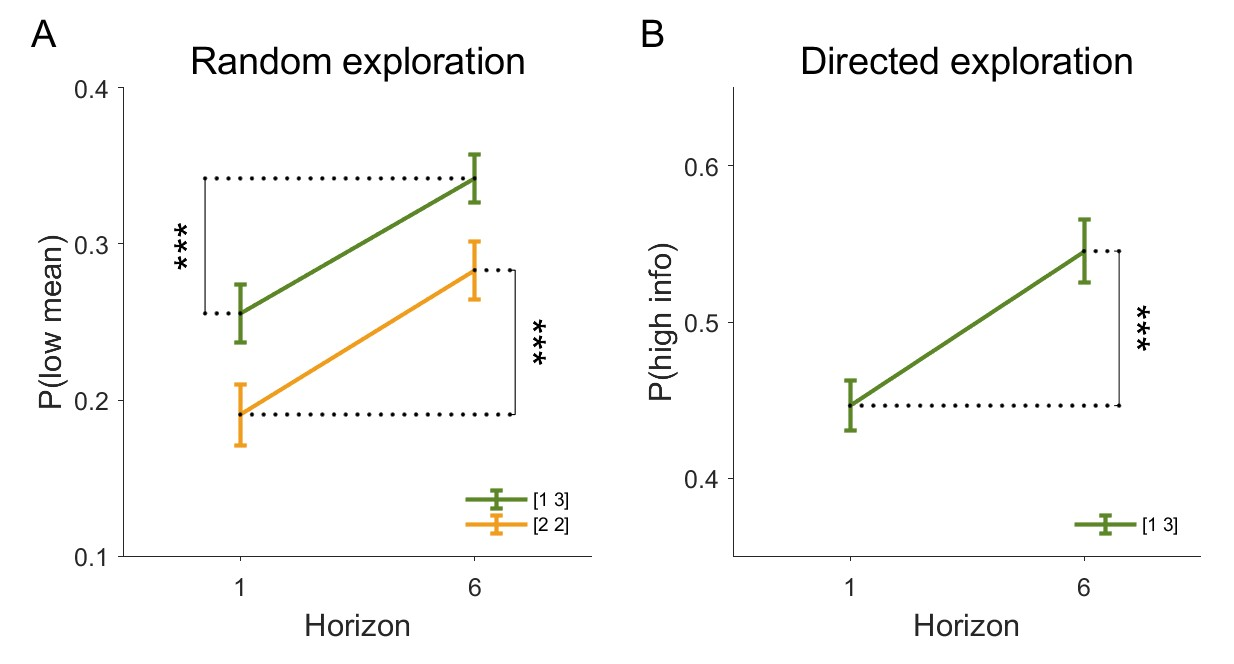
\includegraphics[width=\textwidth]{figures/RanDetNoise_modelfree__all.jpg}
			\caption{Replication of previous findings with data from all participants (i.e. no exclusions). Both  $p(\mbox{low mean})$ (A) and $p(\mbox{high info})$ (B) increase with horizon suggesting that people use both random and directed exploration in this task.  }
			\label{fig:s1}
		\end{center}
	\end{figure}
	\newpage

	\begin{figure}[H]
		\begin{center}
			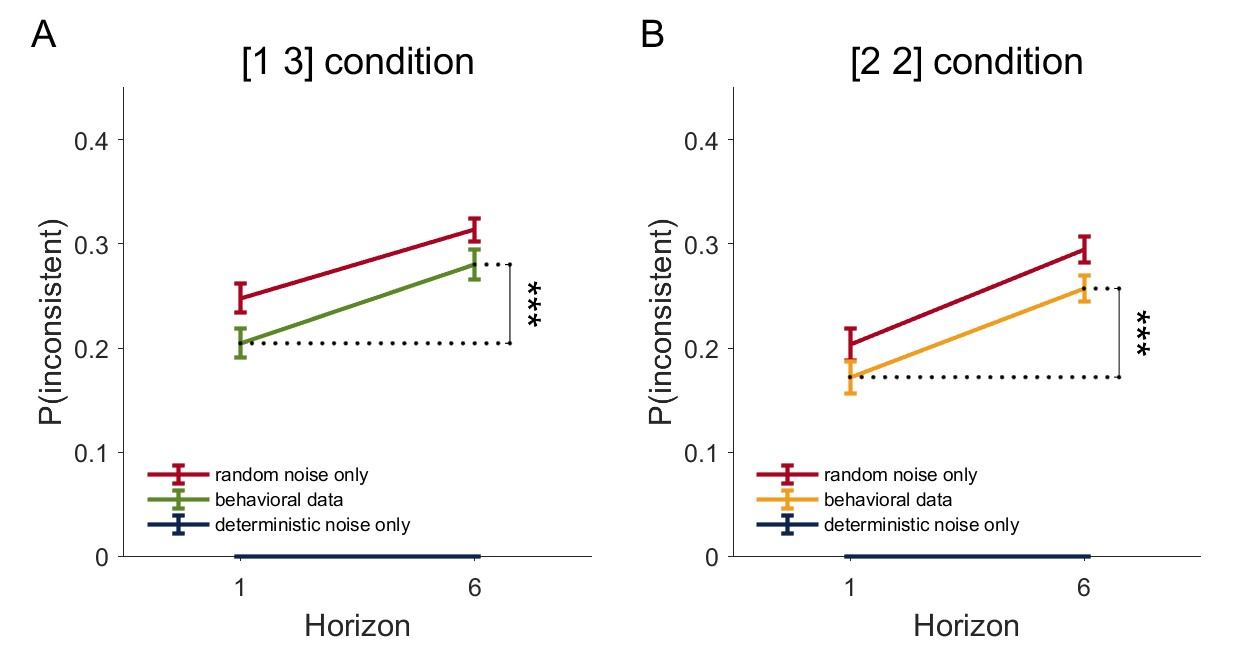
\includegraphics[width=\textwidth]{figures/RanDetNoise_pinconsistent__all.jpg}
			\caption{Model-free analysis with data from all participants (i.e. no exclusions) suggests that both deterministic and random noise contribute to the choice variability in random exploration. For both the [1 3] (A) and [2 2] (B) condition, people show greater choice inconsistency in horizon 6 than horizon 1. However, the extent to which their choices are inconsistent lies between what is predicted by purely deterministic and random noise, suggesting that both noise sources influence the decision.}
			\label{fig:s2}
		\end{center}
	\end{figure}

	\newpage

	\begin{figure}[H]
	\begin{center}
		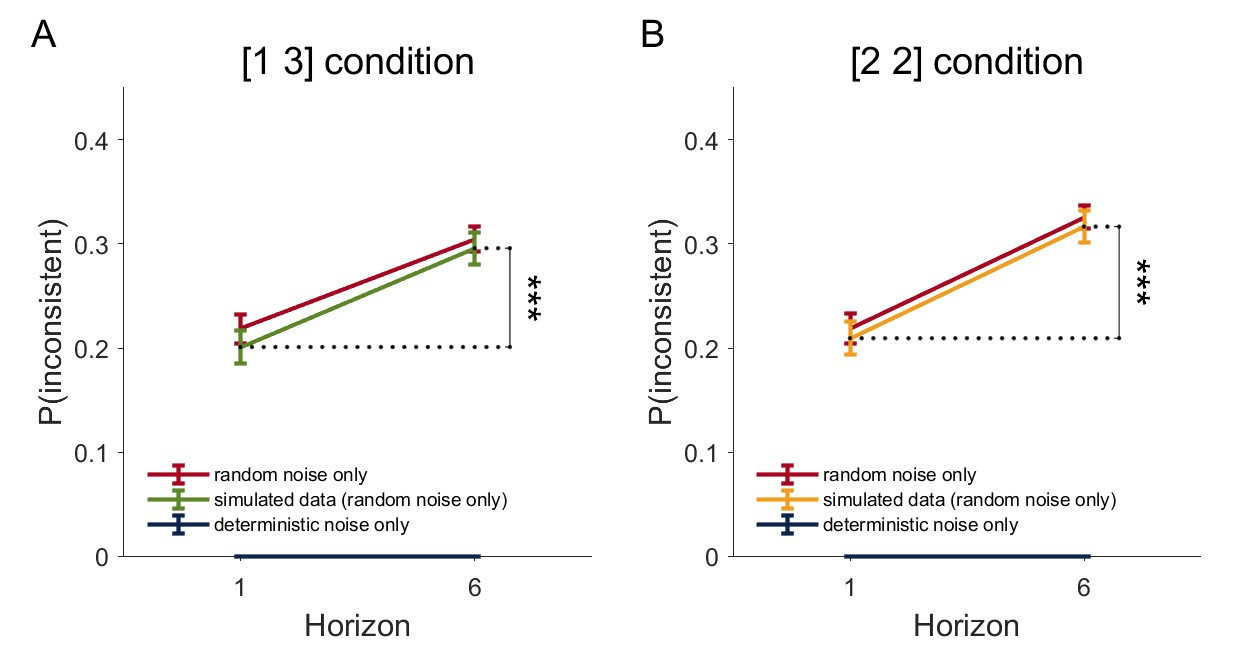
\includegraphics[width=\textwidth]{figures/RDBayes_pinconsistent_validation.jpg}
		\caption{Model-free analysis with simulated choices from a model that has only random noise validates our prediction of p(inconsistent) for pure random noise. The extent to which simulated choices are inconsistent completely overlaps with our pure random noise prediction(p $>$ 0.05). This suggests that when choice inconsistency lies below the pure random noise prediction indeed provides evidence that deterministic noise exists in random exploration (Figure 3).}
		\label{fig:s3}
	\end{center}
	\end{figure}

	\newpage
	\begin{figure}[H]
		\begin{center}
			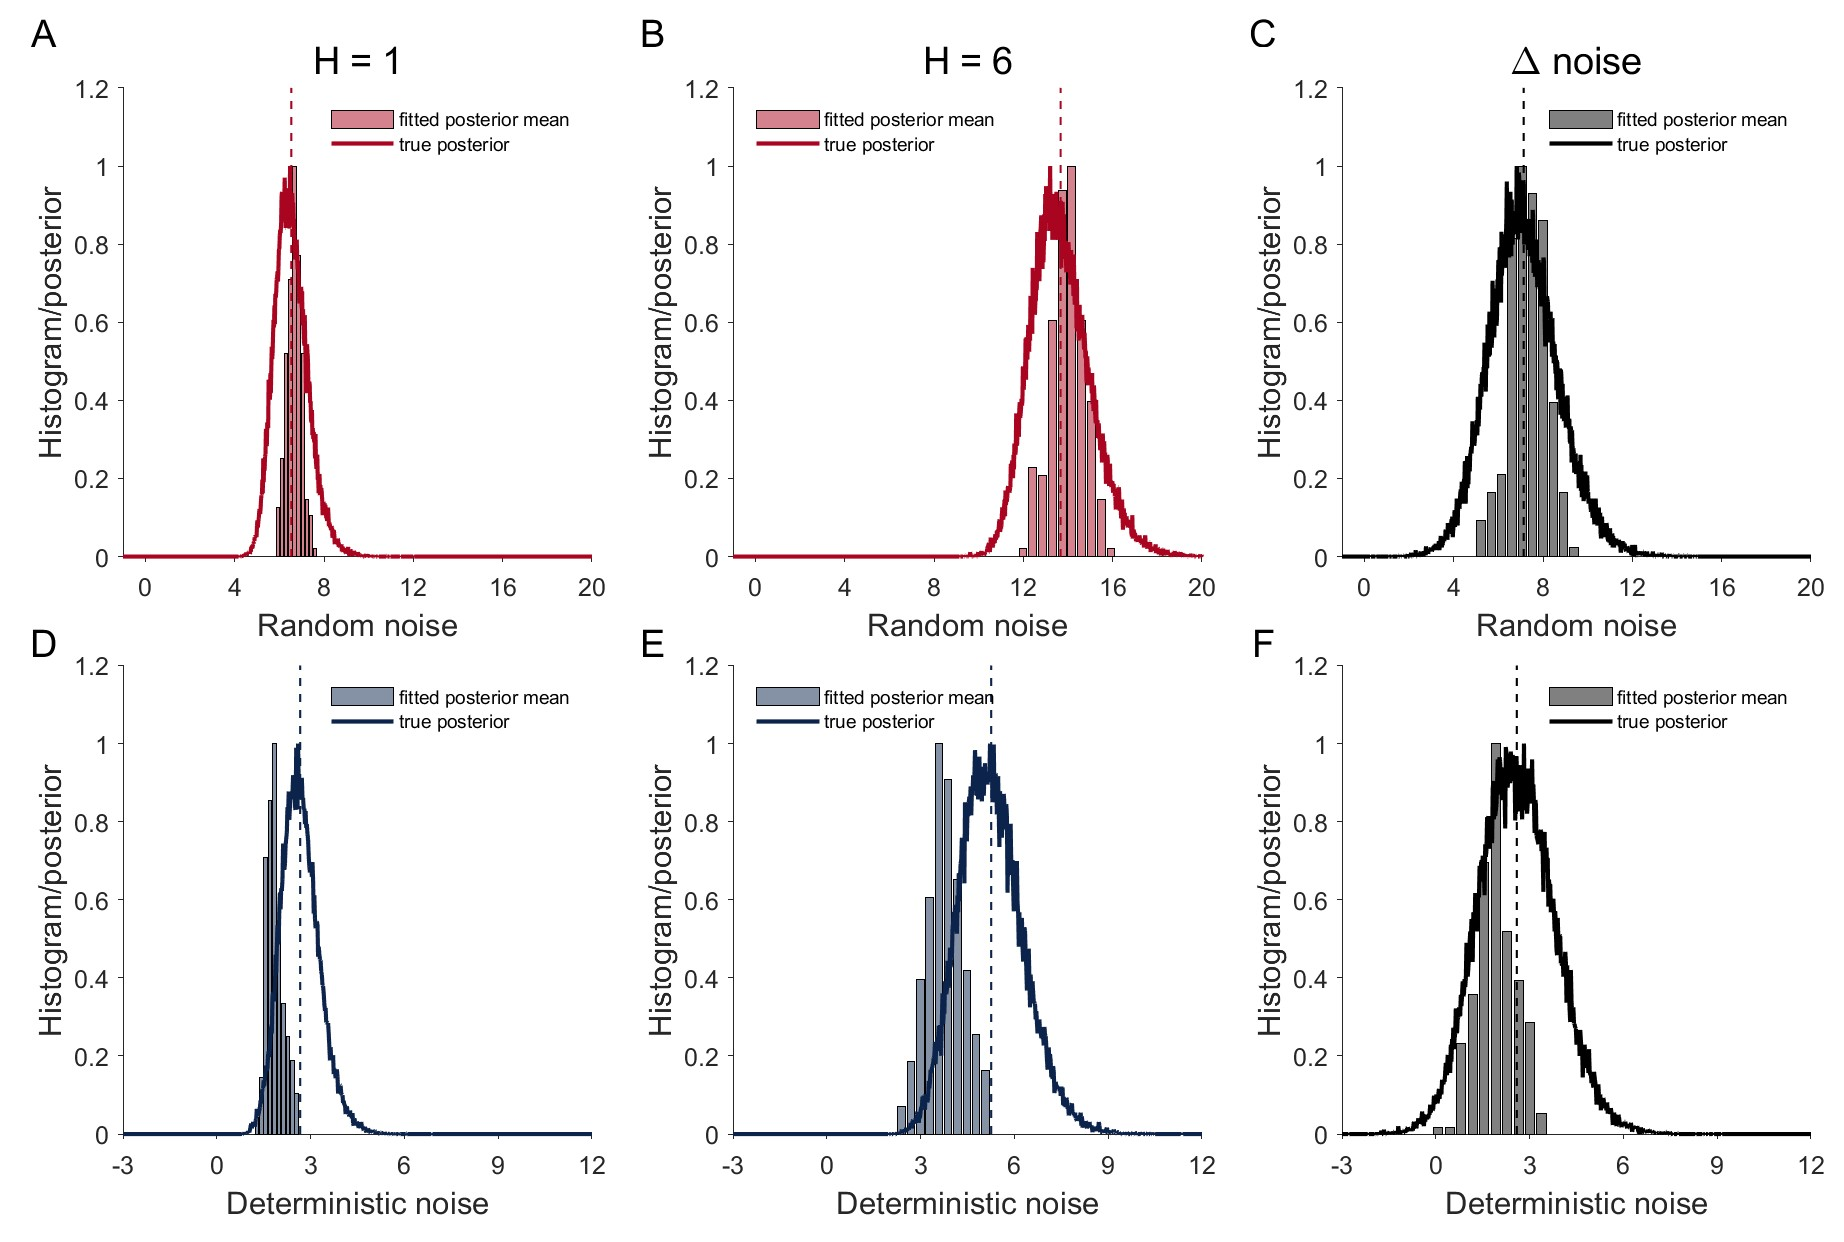
\includegraphics[width=1\textwidth]{figures/RDBayes_parameterrecovery_hyperprior.jpg}
			\caption{Parameter recovery over the mean estimates of random and deterministic noise standard deviations $\sigma_{det}$ and $\sigma_{ran}$. Solid lines are true posterior used to simulate choices, dashed black line is the mean of the true posterior. Histograms represent the mean estimates of the respective parameters in the refitting to the simulated data. (A) and (B) are random noise at H = 1 and H = 6, respectively. (C) is the random noise differences between horizons. (D) and (E) are deterministic noise at H = 1 and H = 6, respectively. (F) is the deterministic noise differences between horizons.}
			\label{fig:s4}
		\end{center}
	\end{figure}

\newpage

	\begin{figure}[hp]
		\begin{center}
			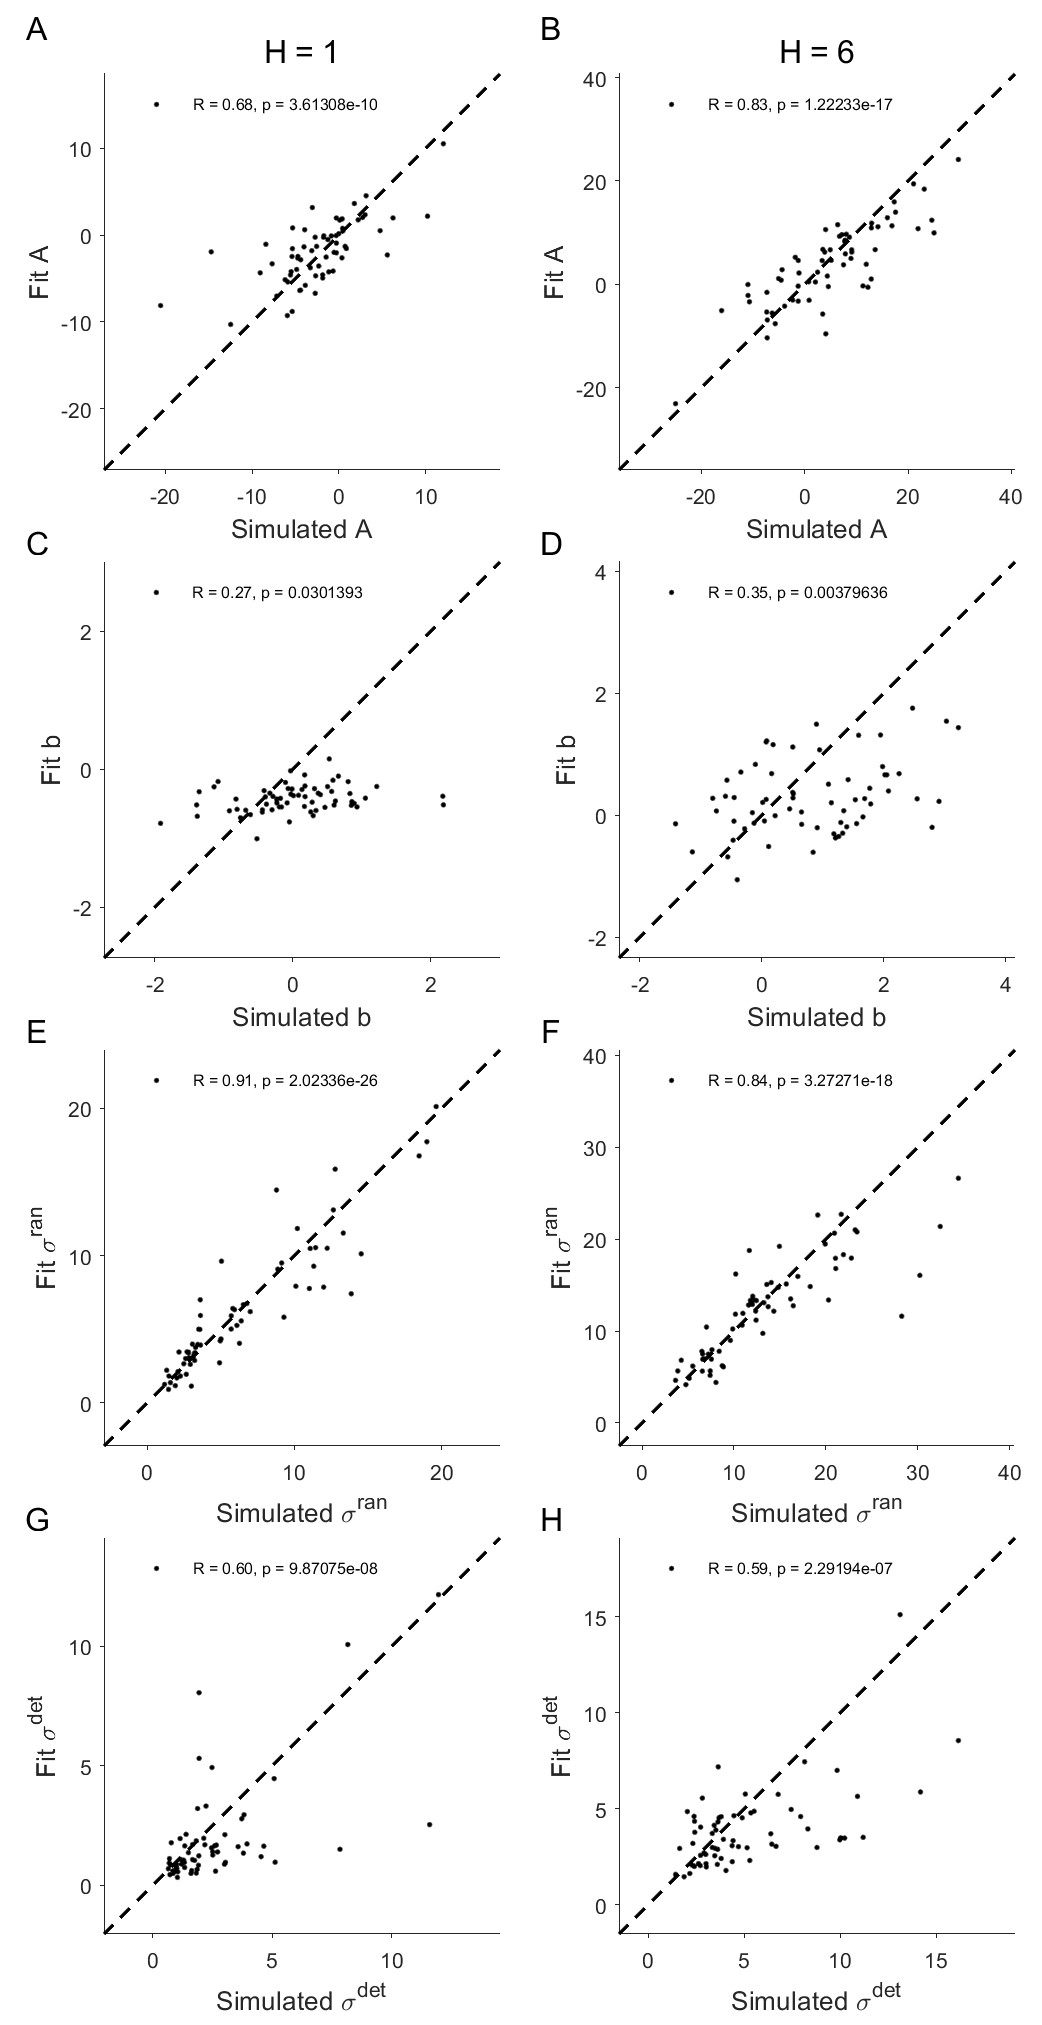
\includegraphics[width=0.6\textwidth]{figures/RDBayes_parameterrecovery_subject_examplesession.jpg}
			\caption{Parameter recovery over the subject-level means of information bonus, $A$, spatial bias, $b$, random noise standard deviation, $\sigma_{ran}$, and deterministic noise standard deviation, $\sigma_{det}$, for horizon 1 (left column) and horizon 6 (right column) games.}
			\label{fig:s5}
		\end{center}
	\end{figure} 
\newpage

	\begin{figure}[hp]
		\begin{center}
			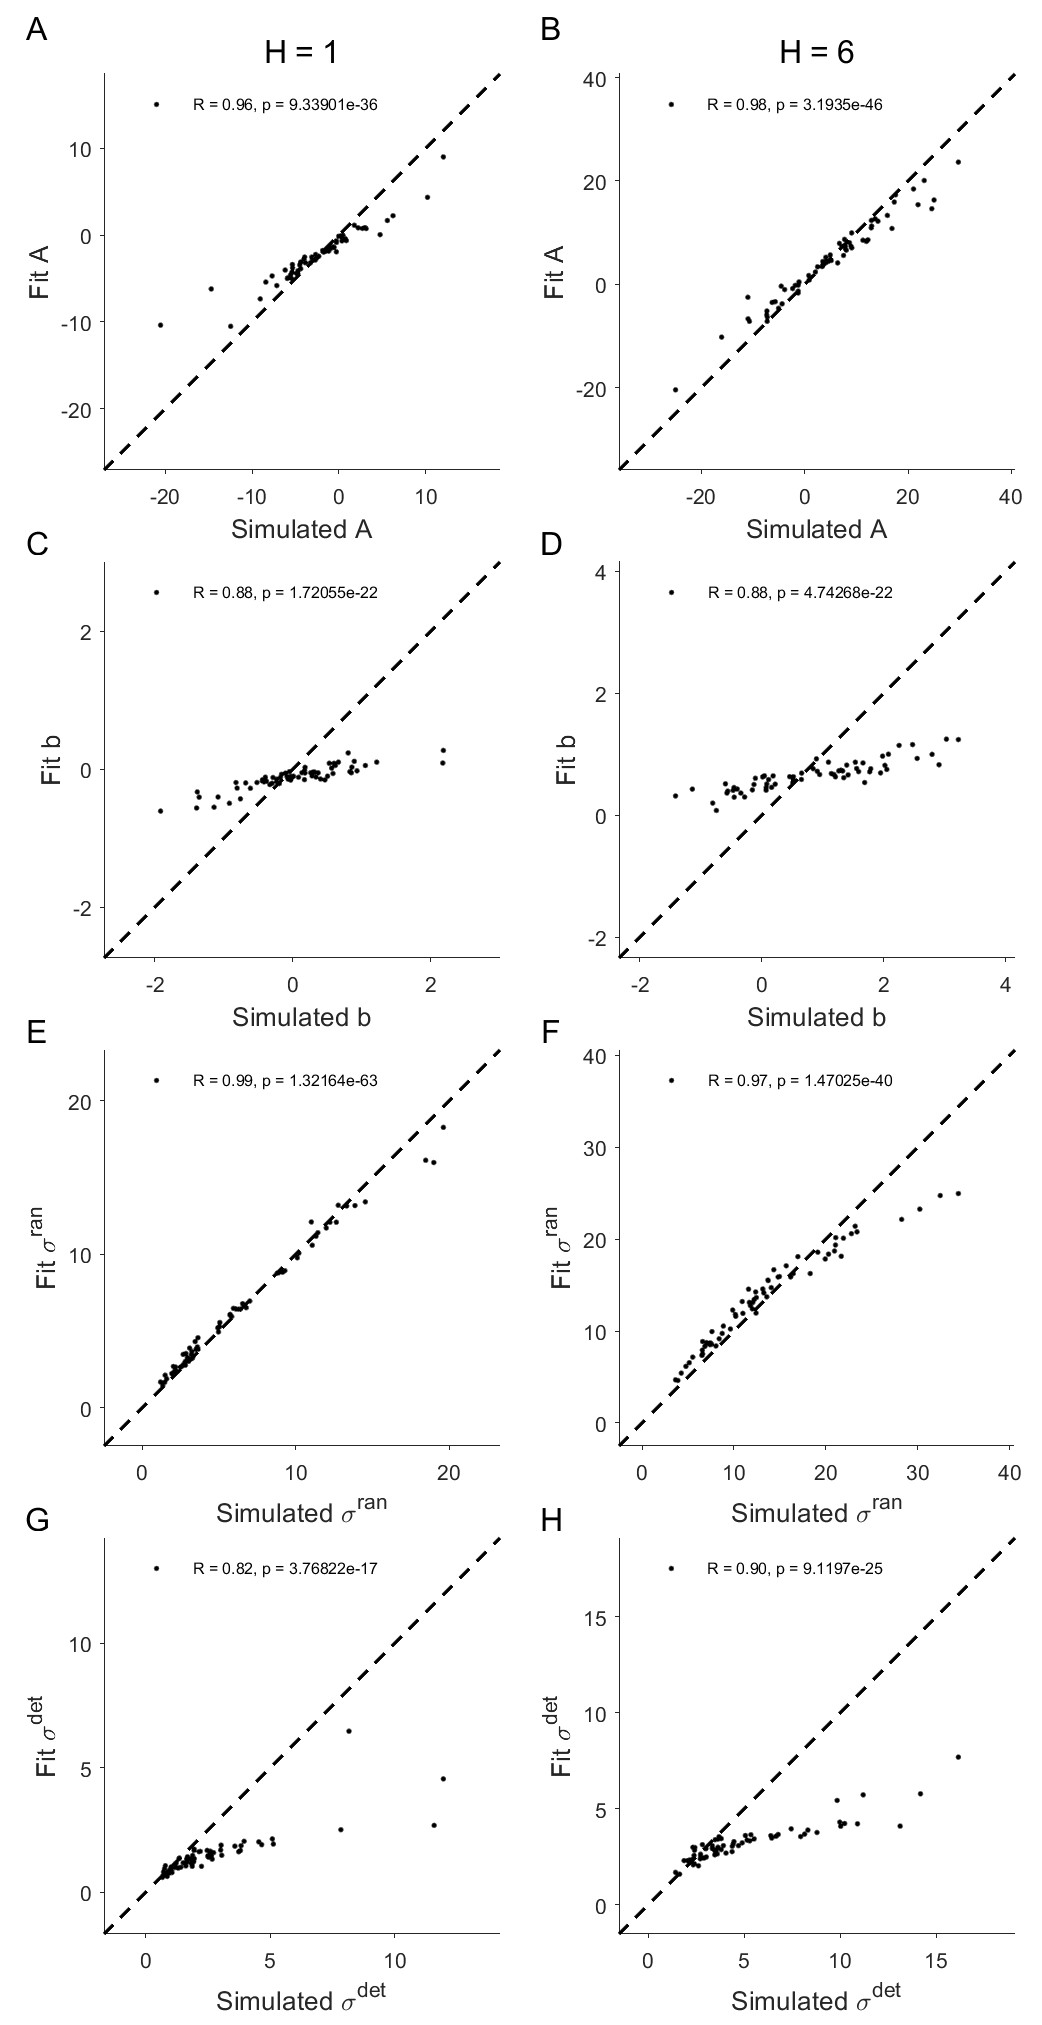
\includegraphics[width=0.6\textwidth]{figures/RDBayes_parameterrecovery_subject.jpg}
			\caption{Same as Supplementary Figure S5, except that the recovered parameters were averaged across 200 repetitions and then compared to the original parameters.}
			\label{fig:s6}
		\end{center}
	\end{figure} 
\newpage


	\begin{figure}[hp]
		\begin{center}
			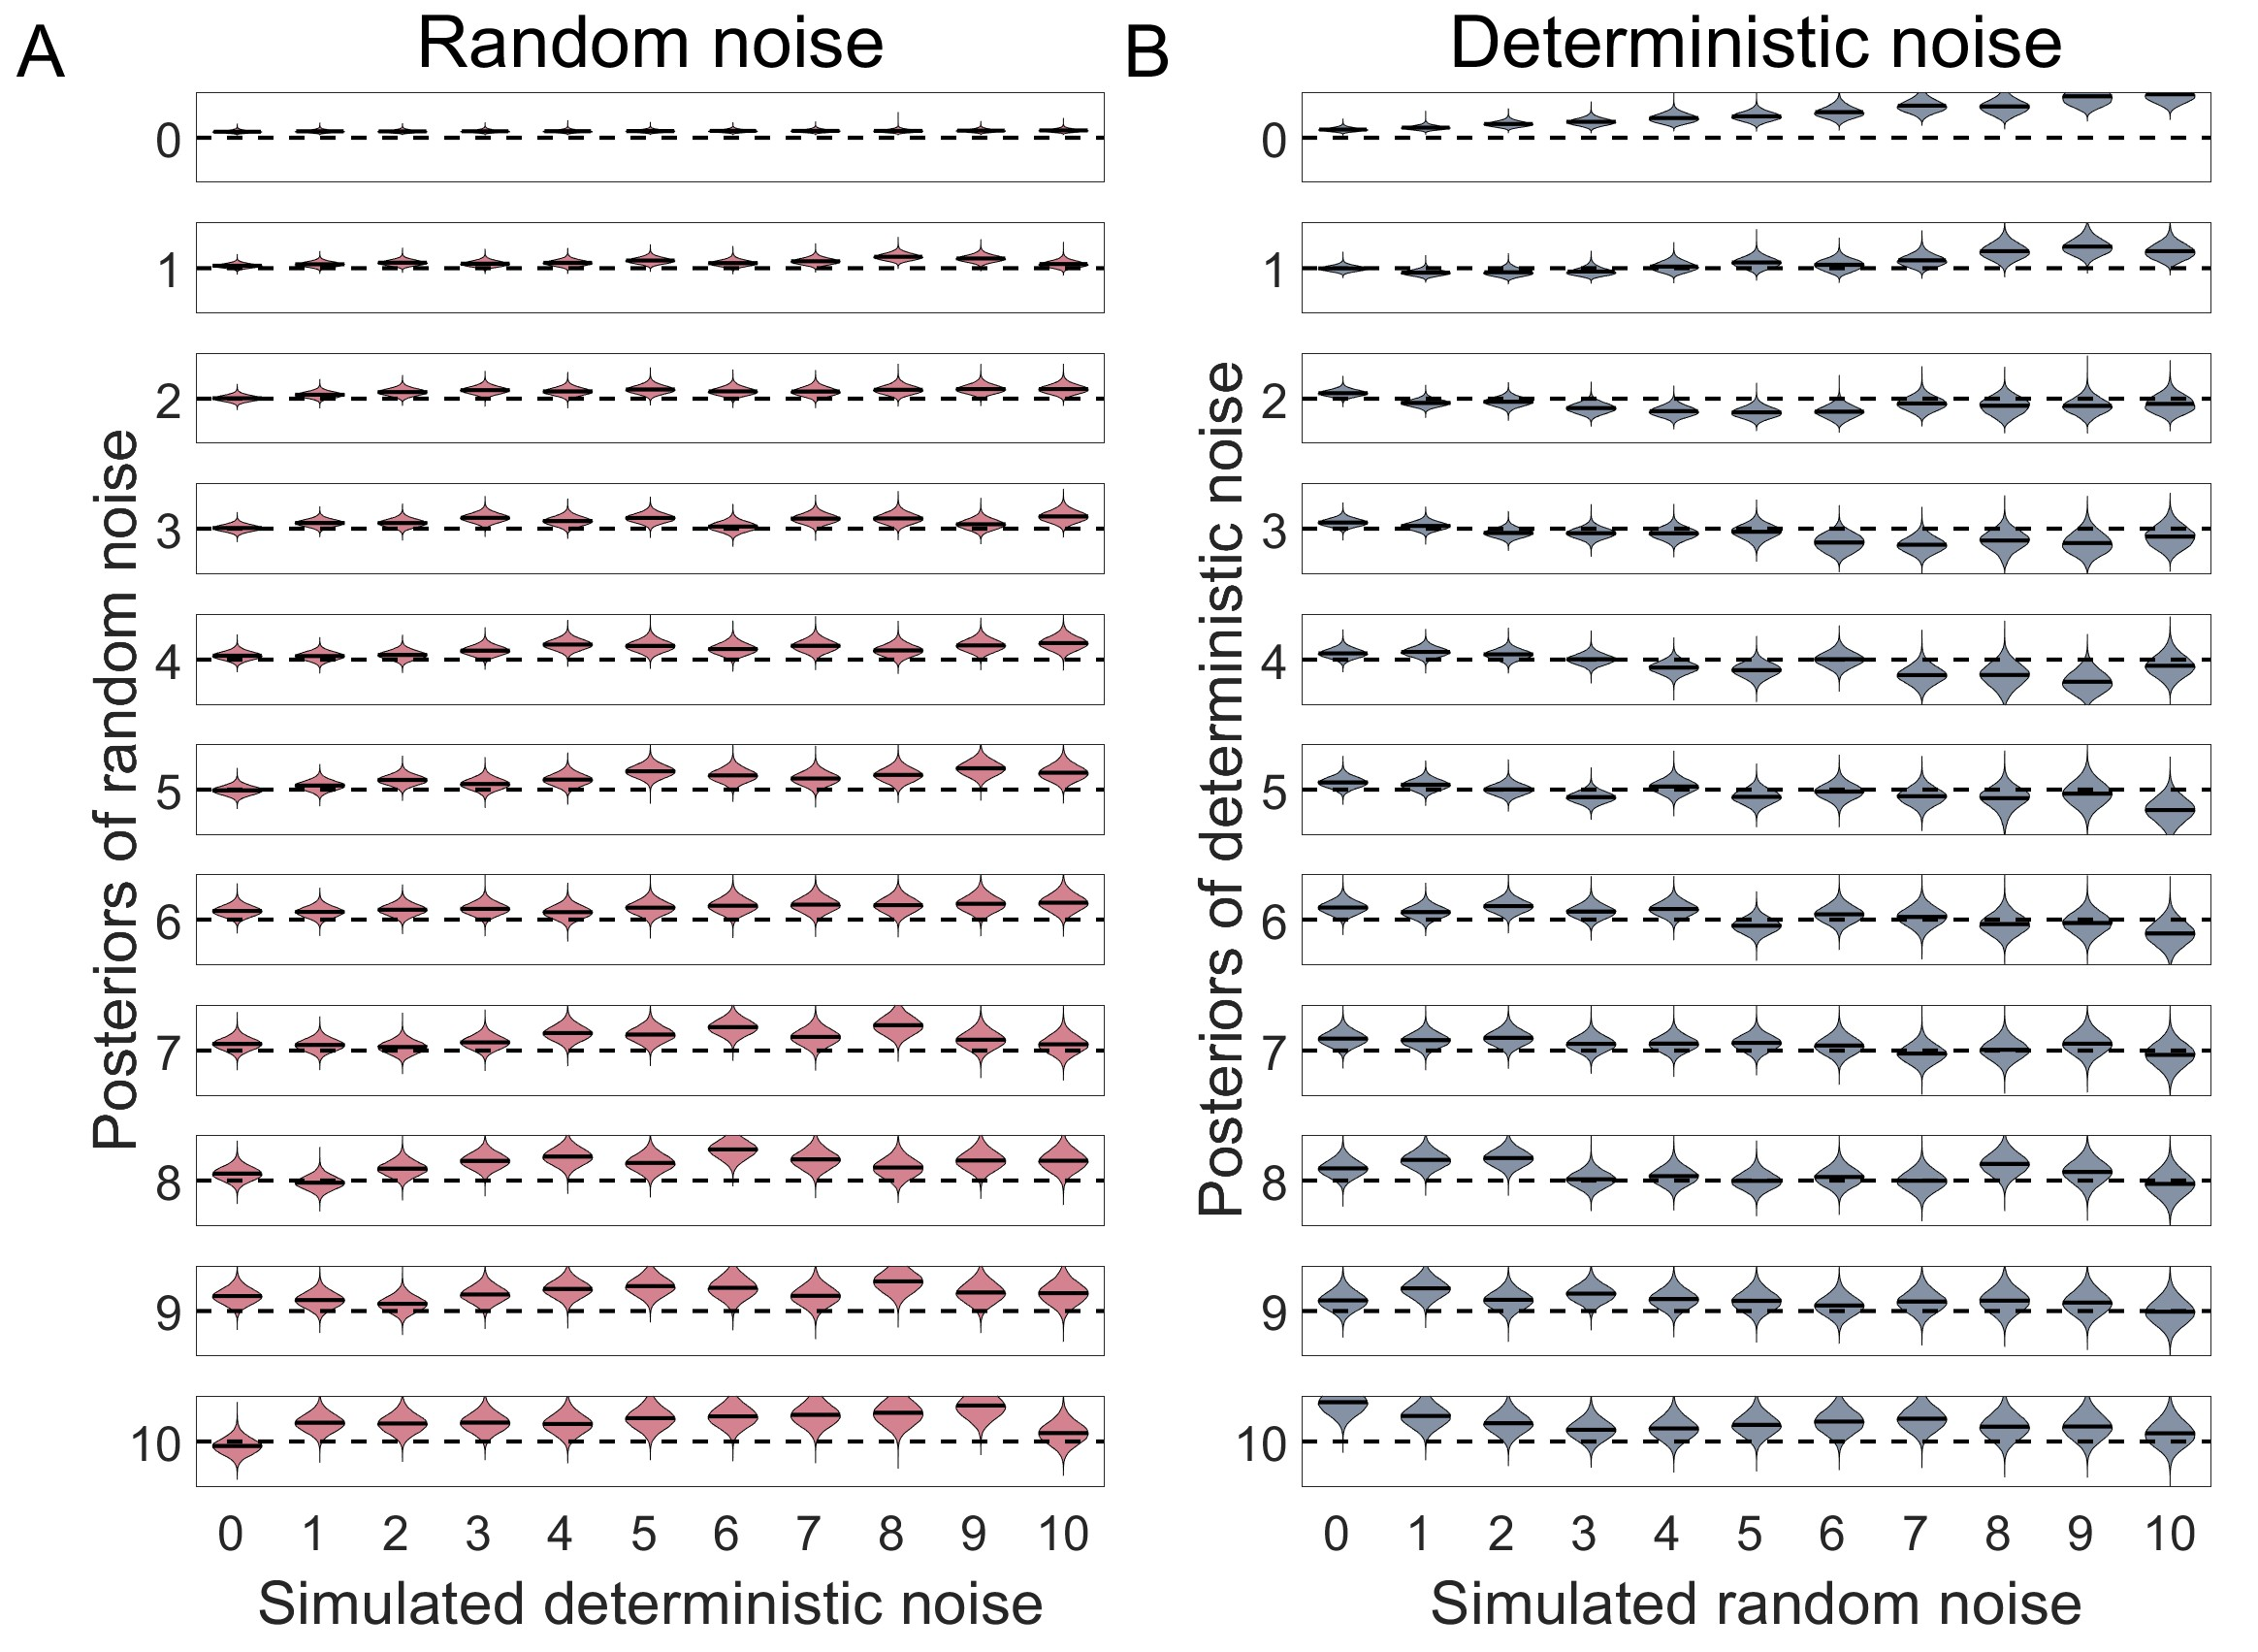
\includegraphics[width=1\textwidth]{figures/RDBayes_parameterrecovery_gridsimu_all.jpg}
			\caption{Parameter recovery on arbitrary combinations of random and deterministic noises. A. Recovered posterior distributions of random noise. B. Recovered posterior distributions of deterministic noise. For both A and B, from the top row to the bottom row, the true noise standard deviation that is used in the simulations go from 0 to 10. The y limit of each panel is 4 (+/- 2 from the true value). Our model did a relatively good job in recovering all combinations of deterministic and random noises.}
			\label{fig:s7}
		\end{center}
	\end{figure} 

	\newpage
	\begin{figure}[H]
		\begin{center}
			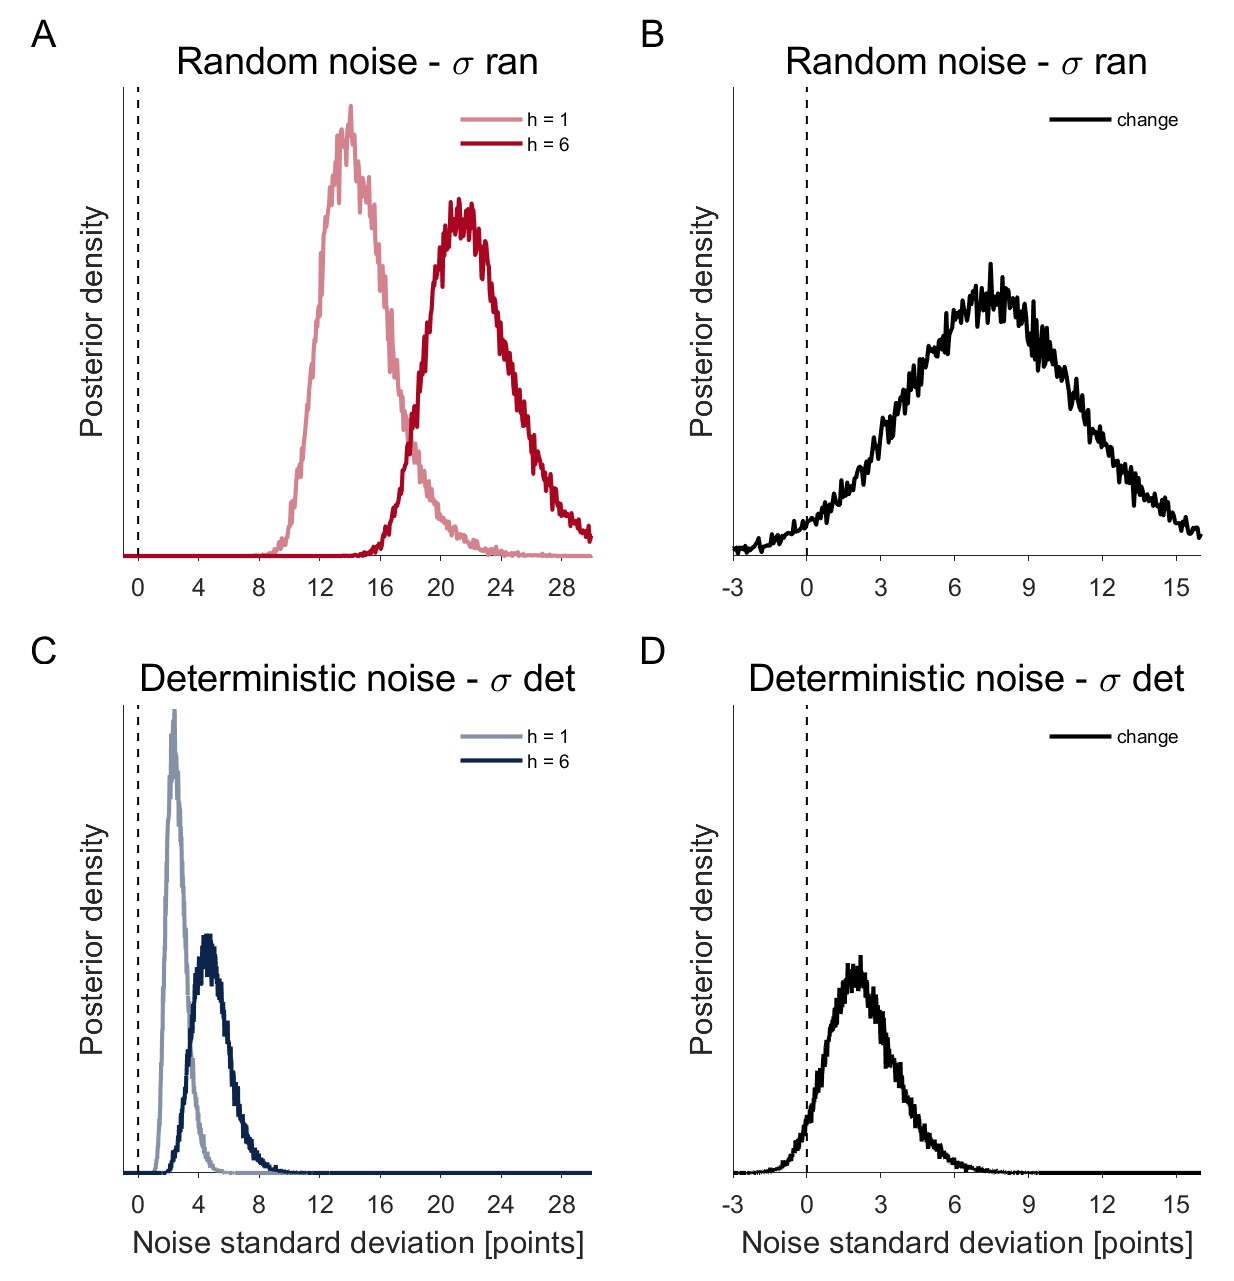
\includegraphics[width=0.7\textwidth]{figures/RDBayes_hyperprior__all.jpg}
			\caption{Model based analysis with data from all participants (i.e. no exclusions) showing the posterior distributions over the group-level mean of the standard deviations of  random and deterministic noise. Both random (A, B) and deterministic (C,D) noises are nonzero (A, C) and change with horizon (B, D).  However, random noise has both a greater magnitude overall (A, C) and a greater change with horizon (B, D) than deterministic noise.}
			\label{fig:s8}
		\end{center}
	\end{figure}
	
	\newpage
	\begin{figure}[t]
		\begin{center}
			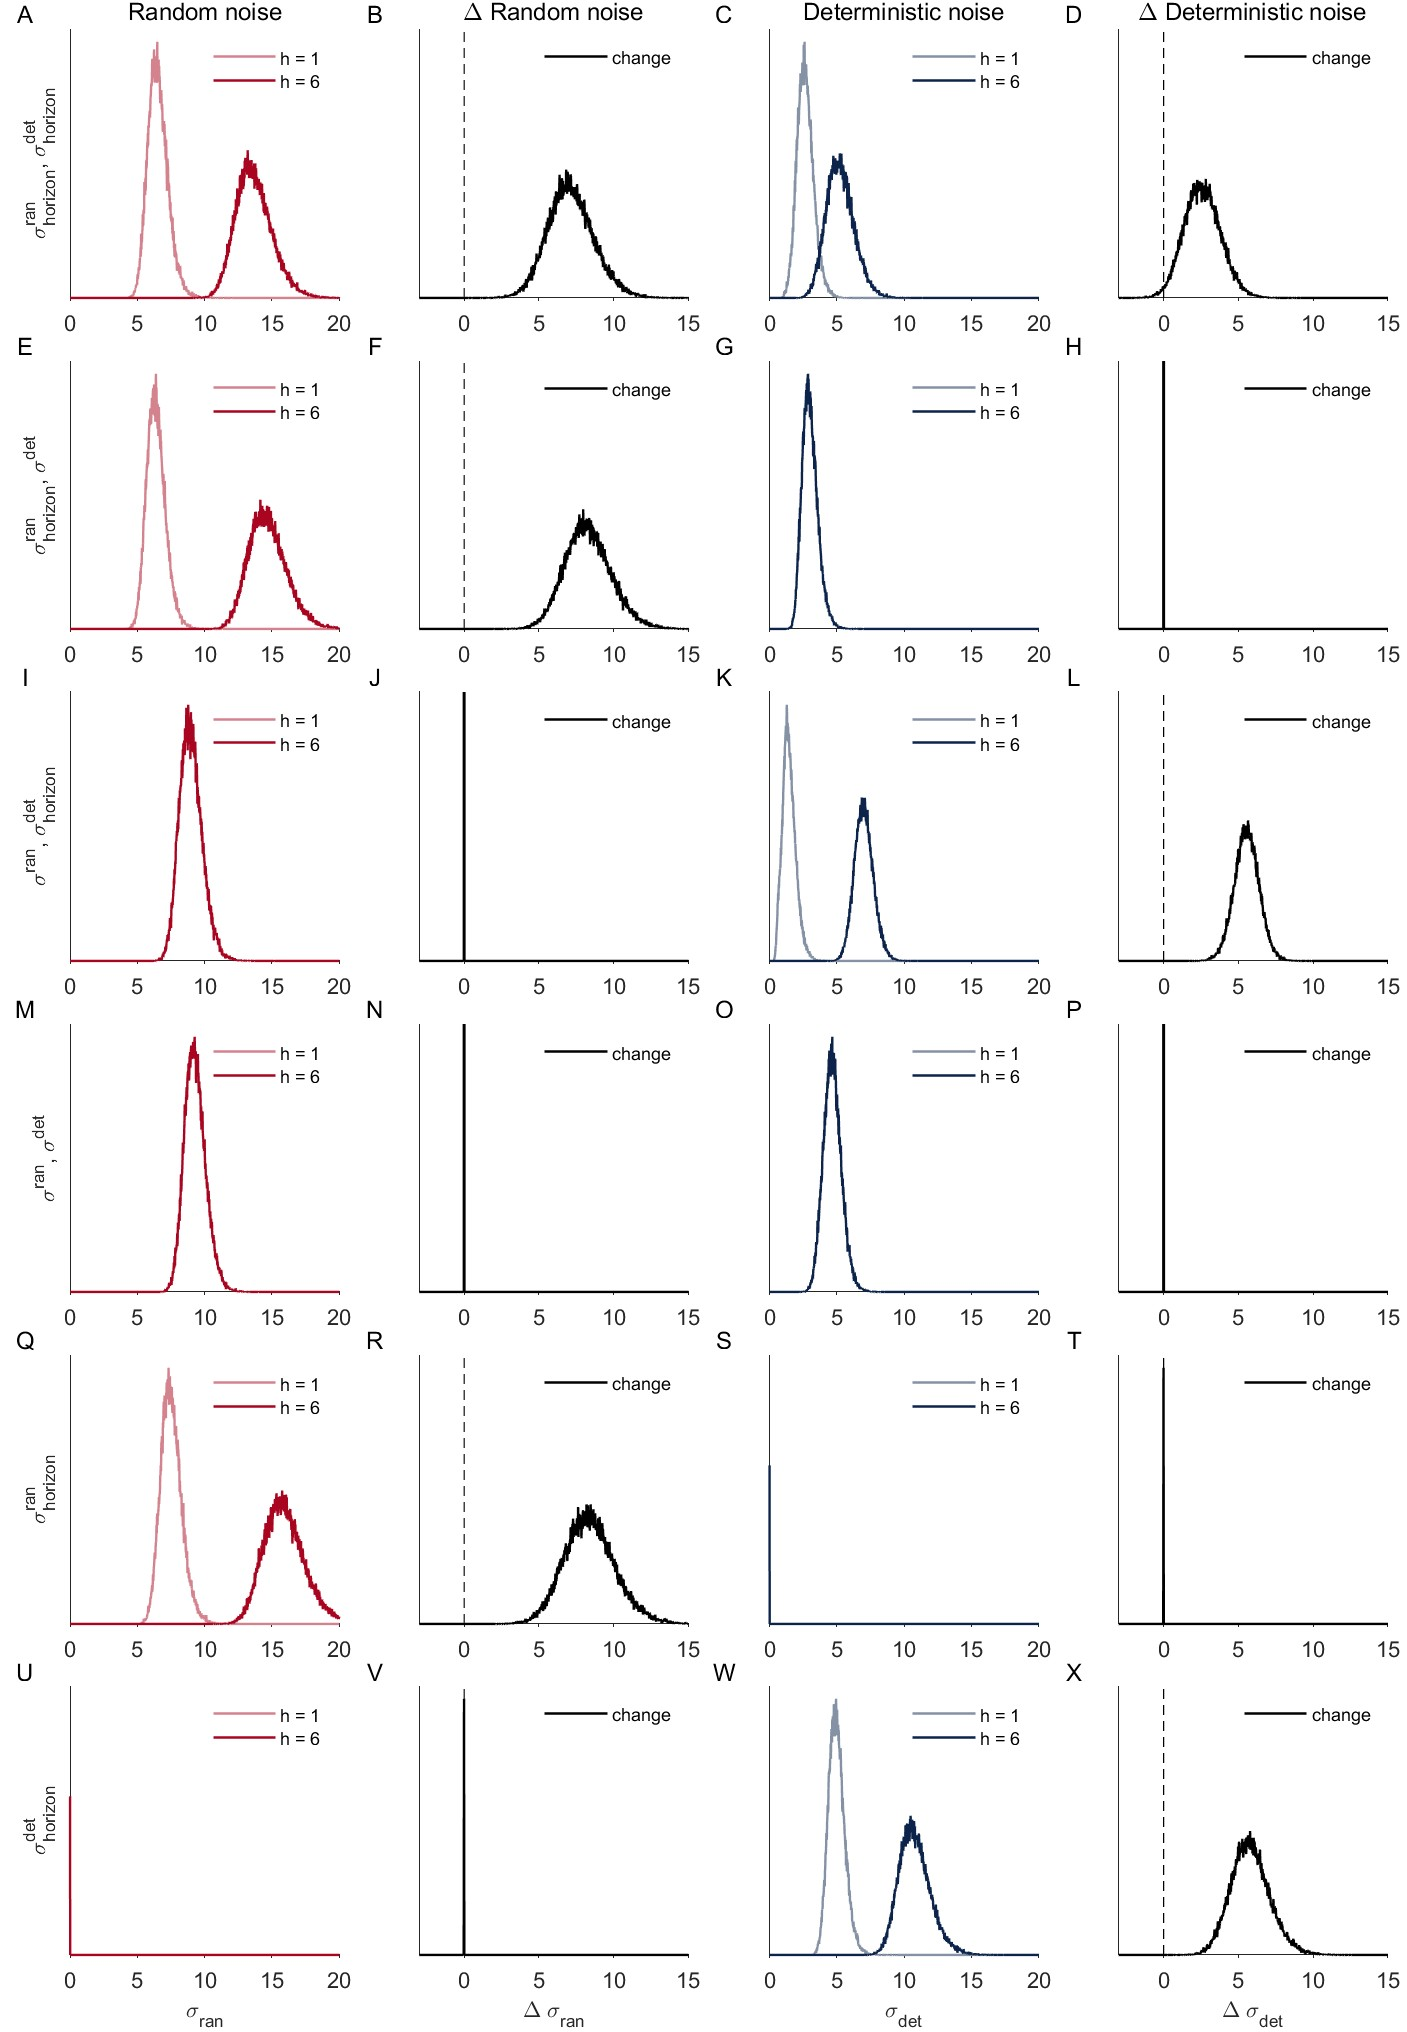
\includegraphics[width=0.8\textwidth]{figures/RDBayes_2noise_hyperpriors_6model.jpg}
			\caption{Model based analysis with variations of models. Each row is one model.  These models varied in whether deterministic $\sigma^{det}$ and random noise $\sigma^{ran}$ are present or not and whether either types of noise is dependent on horizon (subscript denotes the dependence on horizon). }
			\label{fig:s9}
		\end{center}
	\end{figure}

\newpage


	\begin{figure}[hp]
		\begin{center}
			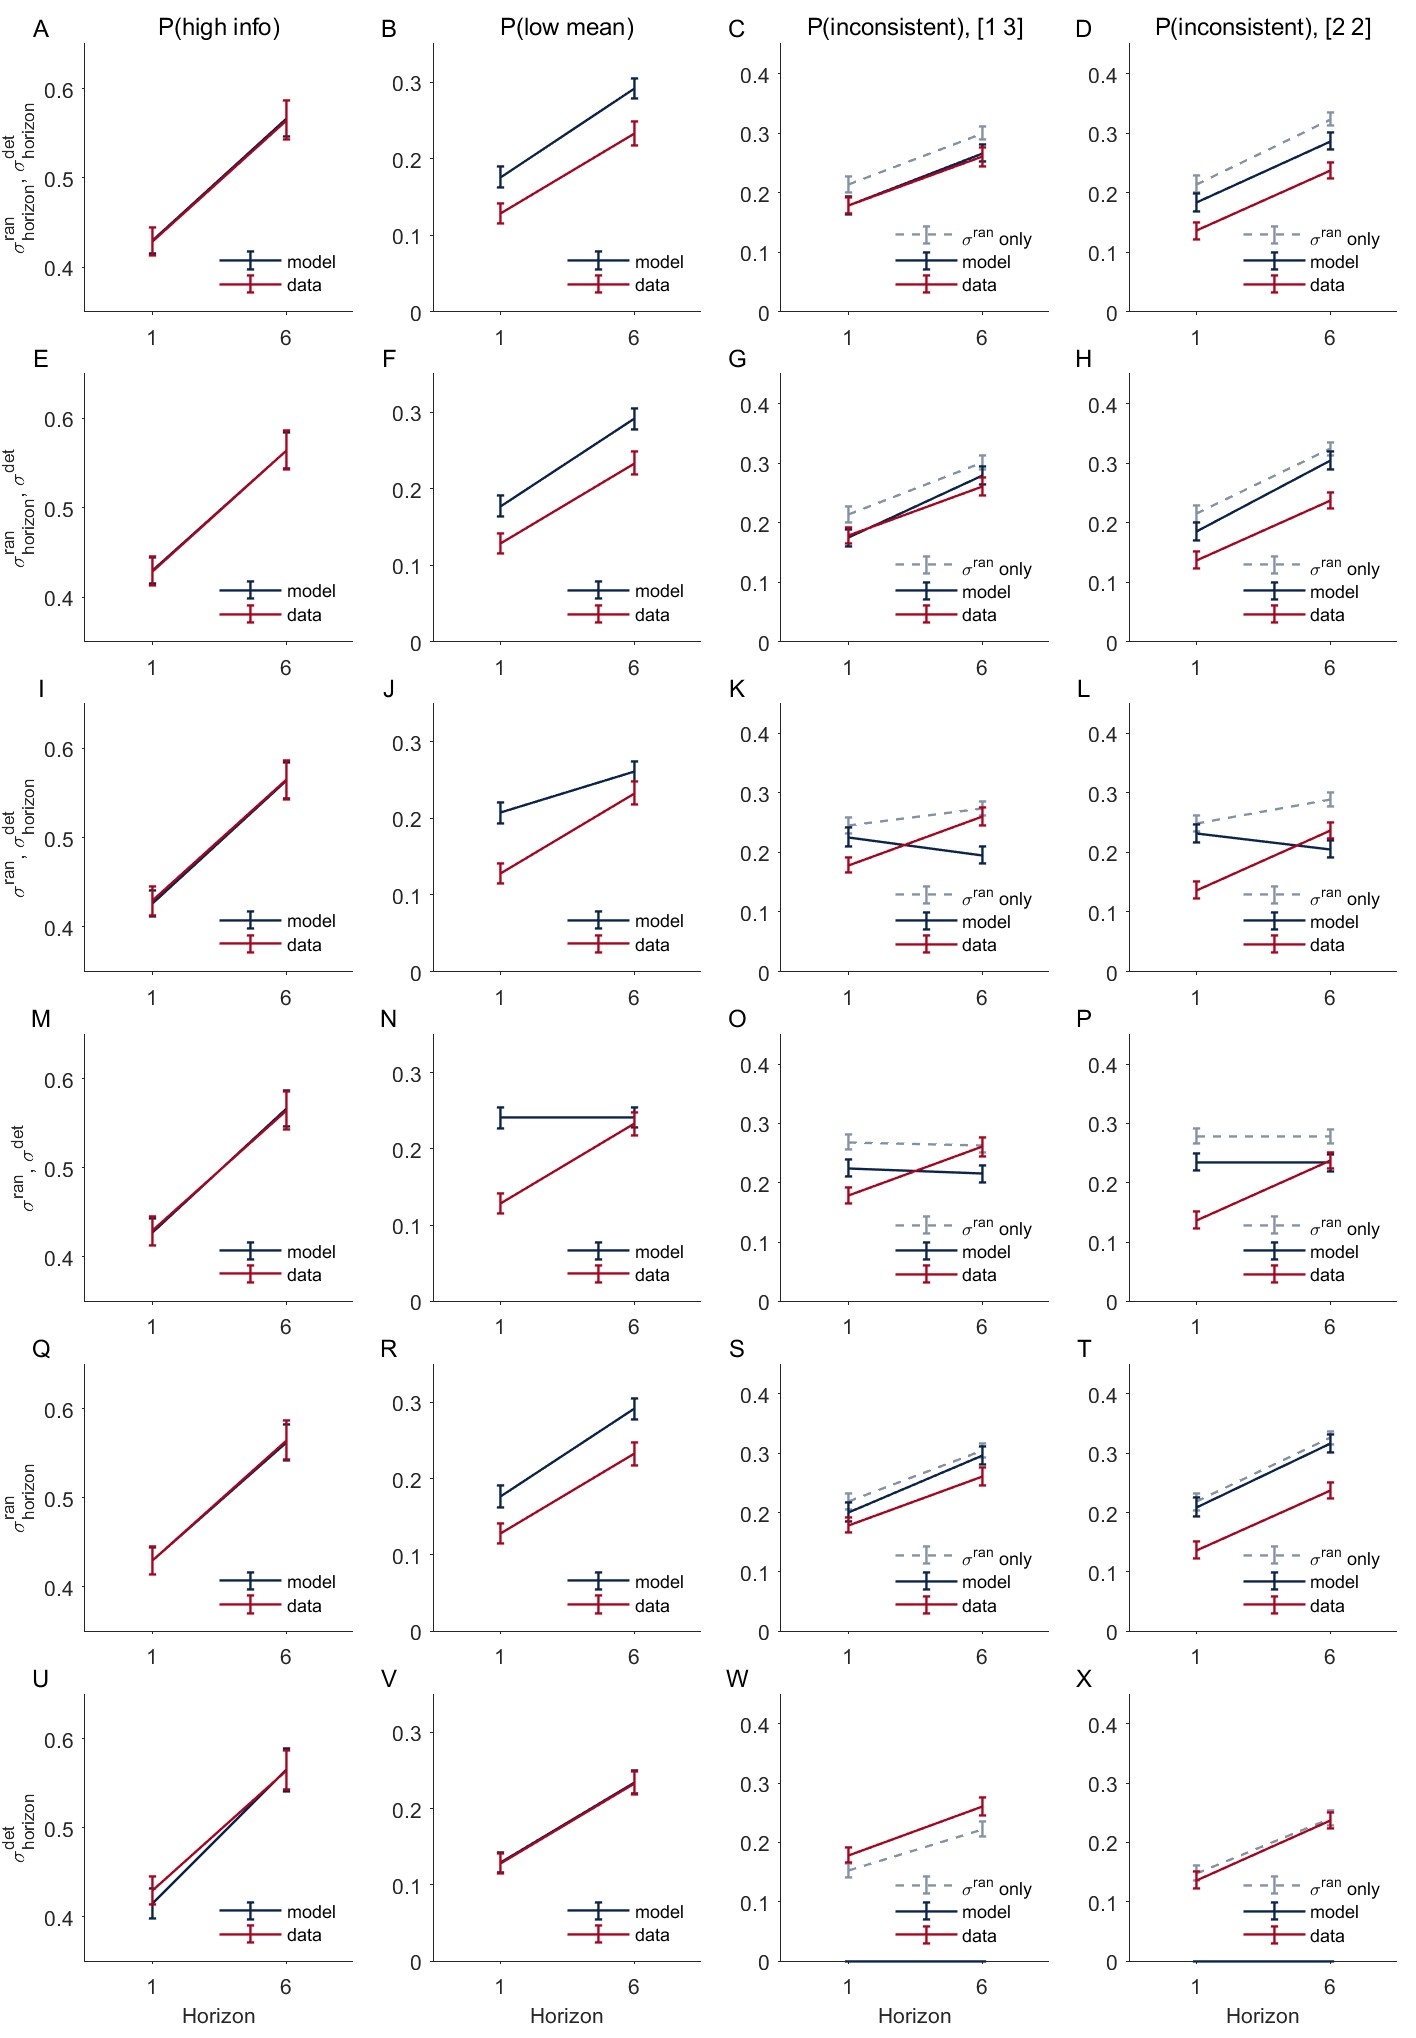
\includegraphics[width=0.8\textwidth]{figures/RDBayes_2noise_6modelcomparison.jpg}
			\caption{
			% BOB SAYS: KEEP THE TOP LINE OF THIS FIGURE FOR THE MAIN PAPER AND MOVE THE FULL FIGURE TO SUPPLEMENTARY MATERIAL TO FIT DESCRIPTION IN TEXT.  
			% ALSO MAKE THE FOLLOWING CHANGES: THIS FIGURE NEEDS A LEGEND IN TOP RIGHT TO SAY WHICH LINE IS MODEL AND WHICH IS NOT.  I WOULD ALSO USE TEXTBOXES (in Matlab annotation('textbox', [0 0 1 1], 'string', 'hi') will get you started) TO DESCRIBE THE MODELS RATHER THAN LABELLING MODEL A ETC ... COULD EVEN HAVE SOME FORM OF TABLE 1 ON THE LEFT HAND SIDE - SO A COLUMN FOR DETERMINISTIC NOISE AND A COLUMN FOR RANDOM NOISE.
			Model comparison. A-D. both deterministic and random noise are horizon dependent, E-H. only random noise is horizon dependent, I-L. only deterministic noise is horizon dependent, M-P. neither random nor deterministic noise is horizon dependent, Q-T. only deterministic noise is assumed to be present, U-X. only random noise is assumed to be present.}
			\label{fig:s10}
		\end{center}
	\end{figure}
\end{document}
